\documentclass[12pt,a4paper]{article}
\usepackage[a4paper,margin=0.8in,footskip=0.25in]{geometry}

\usepackage{graphicx}
\usepackage{subcaption}

\usepackage{mathtools}
\usepackage{physics}

\usepackage{fontspec} % 加這個就可以設定字體
\usepackage{xeCJK} % 讓中英文字體分開設置

\setCJKmainfont{標楷體} % 設定中文的字型,可以直接輸入系統裡有的字型
% \setmainfont{Times New Roman}

\newfontfamily{\Arial}{Arial}
\newfontfamily{\Calibri}{Calibri}
\newfontfamily{\Times}{Times New Roman}

\newCJKfontfamily\Kai{標楷體} % 定義指令\Kai則切換成標楷體
\newCJKfontfamily\Hei{微軟正黑體} % 定義指令\Hei則切換成正黑體
\newCJKfontfamily\NewMing{新細明體} % 定義指令\NewMing則切換成新細明體

\XeTeXlinebreaklocale "zh" % 這二行,中文才能自動換行
\XeTeXlinebreakskip = 0pt plus 1pt

\title{ML Foundation: HW3}
\author{b04902053 鄭淵仁}

\begin{document}
\maketitle
\section{} % 1
\begin{figure}[h!]
	\centering
	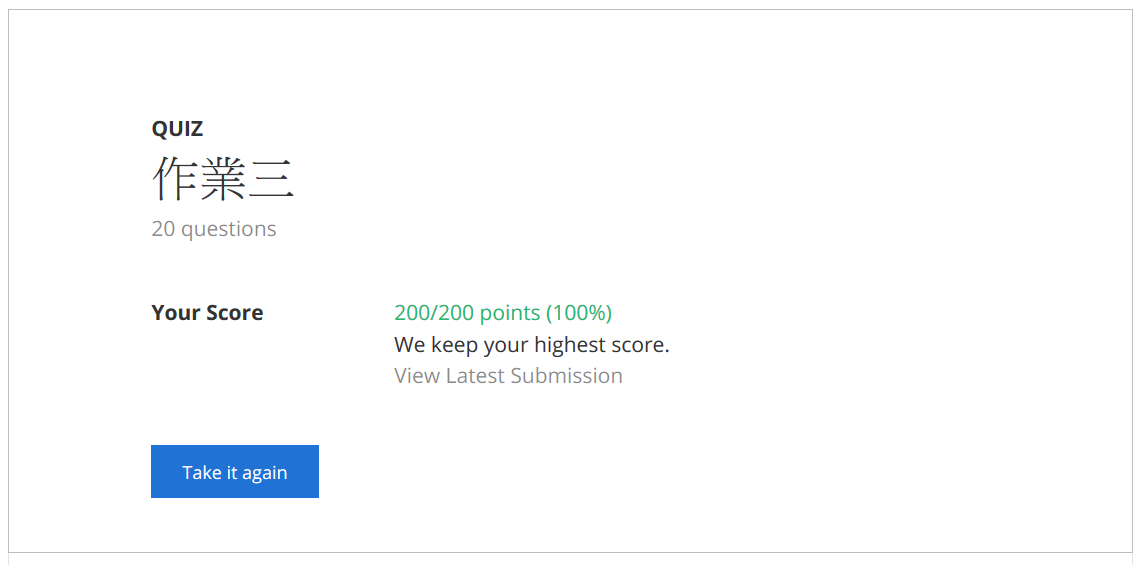
\includegraphics[width=\linewidth]{code/q1.png}
\end{figure}
\section{} % 2
Claim: ${H}^{2} = H$ \\
Proof:
\[
	\begin{aligned}
		{H}^{2} &= {(X {({X}^{T}X)}^{-1} {X}^{T})} ^ {2} \\
				&= (X {({X}^{T}X)}^{-1} {X}^{T}) (X {({X}^{T}X)}^{-1} {X}^{T}) \\
				&= X {({X}^{T}X)}^{-1} [ ({X}^{T} X) {({X}^{T}X)}^{-1} ] {X}^{T} \\
				&= X {({X}^{T}X)}^{-1} {X}^{T} \\
				&= H \\
	\end{aligned}
\]
With the claim above, we can prove that:
\[
	\begin{aligned}
		{(I-H)}^{2} &= {I}^{2} - 2IH + {H}^{2} \\
					&= I - 2H + H \\
					&= I - H \\
	\end{aligned}
\]
\section{} % 3
TODO: 看不懂題目在寫什麼?QQ
\section{} % 4
\[
	\hat{{E}_2}(\Delta u,\Delta v)
		= E(u, v) + \nabla E(u, v) \cdot (\Delta u, \Delta v)
		+ \frac{1}{2} {(\Delta u, \Delta v)}^{T} {\nabla}^{2}E(u, v) (\Delta u, \Delta v)
\]
Set the partial differences of $\hat{{E}_2}(\Delta u,\Delta v)$ be $0$, we have :
\[
	\left\{
		\begin{aligned}
			0 = \pdv{\hat{{E}_2}(\Delta u,\Delta v)}{\Delta u}
				&= \pdv{E}{u} + \frac{1}{2}\left( 2 \pdv[2]{E}{u} \Delta u + 2 \pdv{E}{u}{v} \Delta v \right) \\
				&= \pdv{E}{u} + \pdv[2]{E}{u} \Delta u + \pdv{E}{u}{v} \Delta v \\
			0 = \pdv{\hat{{E}_2}(\Delta u,\Delta v)}{\Delta v}
				&= \pdv{E}{v} + \pdv[2]{E}{v} \Delta v + \pdv{E}{v}{u} \Delta u \\
		\end{aligned}
	\right.
\]
Simplify the equations :
\[
	\left\{
		\begin{aligned}
			0 &= \pdv{E}{u} + \pdv[2]{E}{u} \Delta u + \pdv{E}{u}{v} \Delta v \\
			0 &= \pdv{E}{v} + \pdv[2]{E}{v} \Delta v + \pdv{E}{v}{u} \Delta u \\
		\end{aligned}
	\right.
\]
Now combine the two equations to one equation by vector $(u, v)$ :
\[
	\begin{aligned}
		0 &= \nabla E(u, v) + {\nabla}^{2} E(u, v) \cdot (\Delta u, \Delta v) \\
		- {\nabla}^{2} E(u, v) \cdot (\Delta u, \Delta v) &= \nabla E(u, v) \\
		(\Delta u, \Delta v) &= - {\left({\nabla}^{2} E(u, v)\right)}^{-1} \nabla E(u, v)
	\end{aligned}
\]
Q.E.D.
\section{} % 5
\[
		\max_{h} \prod_{n=1}^{N} h_{y}\left(x_{n}\right) 
		= \max_{w} \prod_{n=1}^{N}
			\frac{\exp({w}_{y_{n}}^{T}x_{n})}{\sum_{k=1}^{K} \exp({w}_{k}^{T}x_{n})}
\]
Take natural log on the it :
\[
	\begin{aligned}
		& \max_{w} \ln \prod_{n=1}^{N}
			\frac{\exp({w}_{y_{n}}^{T}x_{n})}{\sum_{k=1}^{K} \exp({w}_{k}^{T}x_{n})} \\
		&= \max_{w} \sum_{n=1}^{N} \ln
			\frac{\exp({w}_{y_{n}}^{T}x_{n})}{\sum_{k=1}^{K} \exp({w}_{k}^{T}x_{n})} \\
		&= \max_{w} \sum_{n=1}^{N} \left( \ln( \exp({w}_{y_{n}}^{T}x_{n}) ) -
			\ln\sum_{k=1}^{K} \exp({w}_{k}^{T}x_{n}) \right) \\
		&= \min_{w} \sum_{n=1}^{N} \left( \ln\sum_{k=1}^{K} \exp({w}_{k}^{T}x_{n}) -
			{w}_{y_{n}}^{T}x_{n} \right) \\
	\end{aligned}
\]
Therefore the $E_{in}$ is :
\[
	E_{in} = \frac{1}{N} \sum_{n=1}^{N} \left( \ln \sum_{k=1}^{K} \exp({w}_{k}^{T}x_{n}) -
		{w}_{y_{n}}^{T}x_{n} \right) \\
\]
\section{} % 6
First we compute :
\[
	\begin{aligned}
		& \pdv{\left(\sum_{n=1}^{N} \left( \ln\sum_{k=1}^{K}
			\exp({w}_{k}^{T} x_{n})\right)\right)}{w_{i}} \\
		&= \sum_{n=1}^{N} \left( \frac{\exp({w}_{i}^{T} x_{n})}
			{\sum_{k=1}^{K} \exp({w}_{k}^{T} x_{n})}x_{n} \right) \\
		&= \sum_{n=1}^{N} \left( h_{i}(x_{n}) x_{n} \right) \\
	\end{aligned}
\]
Therefore the answer is :
\[
	\begin{aligned}
		\pdv{E_{in}}{w_{i}}
			&= \pdv{\left(\frac{1}{N} \sum_{n=1}^{N} \left( \ln \sum_{k=1}^{K} \exp({w}_{k}^{T}x_{n}) -
			{w}_{y_{n}}^{T}x_{n} \right) \right)}{w_{i}} \\
		&= \frac{1}{N} \sum_{n=1}^{N} \left( \left( h_{i}(x_{n}) x_{n} \right) -
			[[y_{n}=i]] x_{n} \right) \\
		&= \frac{1}{N} \sum_{n=1}^{N} \left( \left( \left( h_{i}(x_{n}) \right) -
			[[y_{n}=i]] \right) x_{n} \right) \\
	\end{aligned}
\]
\section{} % 7
\begin{figure}[h!]
	\centering
	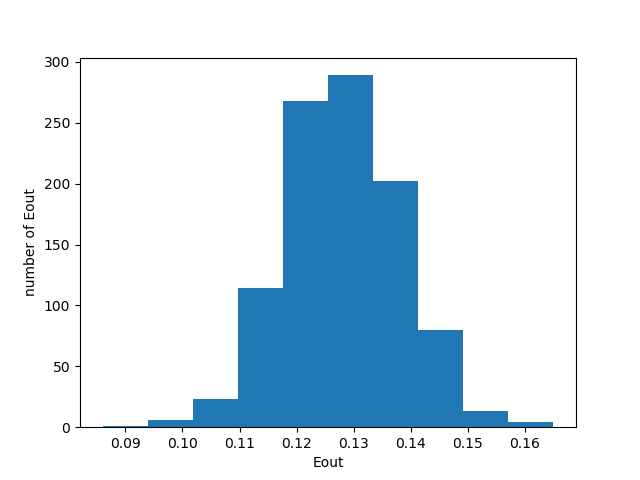
\includegraphics[width=0.8\linewidth]{code/q7.png}
	\caption{Histogram of ${E}_{out}$}
	\label{fig:q7}
\end{figure}
Figure \ref{fig:q7} shows the histogram of ${E}_{out}$.
\section{} % 8
\begin{figure}[h]%
	\begin{subfigure}[h]{0.45\textwidth}
		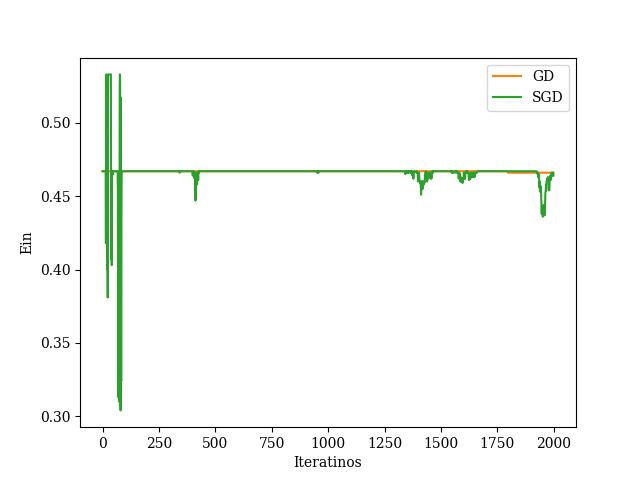
\includegraphics[width=\textwidth]{code/q8_001.png}
		\caption{$lr=0.001$}
	\end{subfigure}
	\hfill\vrule\hfill
	\begin{subfigure}[h]{0.45\textwidth}
		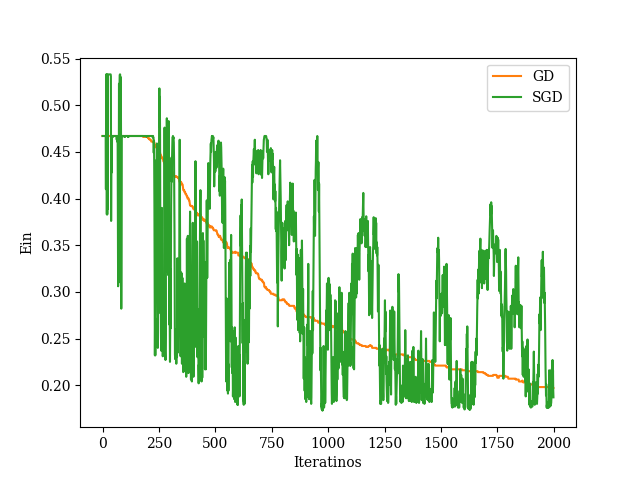
\includegraphics[width=\textwidth]{code/q8_01.png}
		\caption{$lr=0.01$}
	\end{subfigure}%
	\caption{Comparison between $GD$ and $SGD$ in $E_{in}$.}
	\label{fig:q8}
\end{figure}
My findings:
\begin{itemize}
	\item $GD$ 和 $SGD$ 的差異: \\
	我發現 $GD$ 的 $E_{in}$ 很快就會穩定保持相同,或是穩定下降,而不會上下亂跳;相較之下, $SGD$ 的 $E_{in}$ 則是很容易上下浮動。 \\
	我想這是因為 $SGD$ 一次只會取一筆資料來計算 gradient ,如果這一筆資料有 noise 的話,算出來的 gradient 很容易會被 noise 影響;相較之下, $GD$ 一次會用所有資料來計算 gradient ,依照 Hoeffding's Inequality 可以知道:取愈多資料,平均的 noise 有越高的機率會愈小,所以才會有這樣的結果。
	\item $lr = 0.001$ 和 $lr = 0.01$ 的差異: \\
	我發現 $lr = 0.001$ 的時候,除了剛開始 $E_{in}$ 不穩定亂跳以外,
\end{itemize}
\section{} % 9
\begin{figure}[h]%
	\begin{subfigure}[h]{0.45\textwidth}
		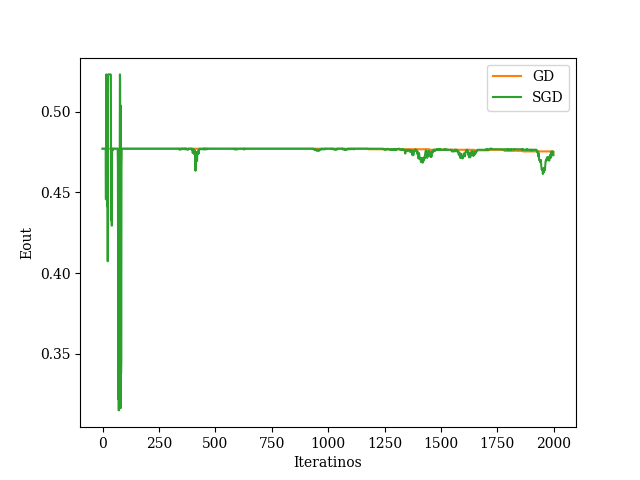
\includegraphics[width=\textwidth]{code/q9_001.png}
		\caption{$lr=0.001$}
	\end{subfigure}
	\hfill\vrule\hfill
	\begin{subfigure}[h]{0.45\textwidth}
		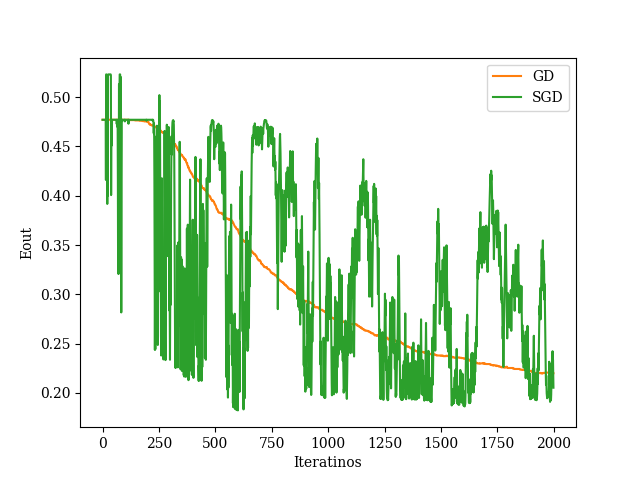
\includegraphics[width=\textwidth]{code/q9_01.png}
		\caption{$lr=0.01$}
	\end{subfigure}%
	\caption{Comparison between GD and SGD in $E_{out}$.}
	\label{fig:q9}
	% 結果和 $E_{out}$ 很像,所以如果可以把最小值紀錄下來,結果應該會更好
\end{figure}
\end{document}
